\section{Datensatzlehre}

\subsection{Datensatzformate}

Basierend darauf welcher Objektdetektor trainiert werden soll, muss der zum Training verwendete Datensatz in einem bestimmten Format vorliegen. Zum Trainieren des \textit{SSDs} wird das sogenannte \textit{Pascal Visual Object Classes} (PascalVOC) Format benötigt. 

Es definiert eine Unterteilung in \textit{Annotations}, \textit{ImageSets} und \textit{JPEGImages}. Während in dem Ordner \textit{JPEGImages} alle Bilder des Datensatzes vorhanden sind, befindet sich unter anderem die Information über die vorhandenen Objekte in dem Bild im Ordner \textit{Annotations}. Für jedes Bild des Datensatzes werden die Informationen in einer gleichnamigen XML-Datei abgelegt. 

\lstset{language=XML}
\lstinputlisting[
label=pascalvoc:PascalVOC,
caption=pascalVOC Bildannotation,
captionpos=b,
firstline=1,
lastline=26
]{Quellcode/annotation.xml}

Neben allgemeinen Metainformationen über das Bild befindet sich hier ebenso eine Liste aller markierten Objekte. Pro Objekt wird die Klassifikationskategorie, die Ausrichtung (z.B. \glqq Frontal\grqq{}), die Information über vollständiges Erscheinen im Bild, die Information über schwere Erkennbarkeit und die Bounding Box angegeben. Im Ordner \textit{ImageSets/Main} wird eine Unterteilung in Trainings- und Testdatensatz durch zwei Textdateien realisiert, die die Dateinamen der Bilddateien als Auflistung enthalten. \cite{RenuKhandelwal.2019}

Das \textit{YOLO} Format für den \textit{YOLO} Objektdetektor definiert in einer \textit{.names}-Datei alle im Datensatz vorhandenen Kategorien durch simple Auflistung der Bezeichner. Die Bilder werden zusammen mit ihren Annotationen in einem separaten Ordner abgelegt. Die Annotationen folgen hier dem Format:

$<Kategorie-ID>\:<Zentrum-X>\:<Zentrum-Y>\:<Breite>\:<Hoehe>$

Die Unterteilung in Trainings- und Testdatensatz erfolgt durch Referenzierung der Bildpfade in zwei getrennten Textdateien. Schließlich wird in einer \textit{.data}-Datei der Pfad zu den beiden Textdateien und zur \textit{.names}-Datei sowie die Anzahl an Kategorien gespeichert. \cite{ArunPonnusamy.20191006}

\subsection{Datensatzzusammensetzung}

Zum Erstellen und Auswählen eines \textit{Deep Learning} Modells wird der Datenbestand in der Regel in drei Kategorien unterteilt. Ein Datensatz wird für das Training des Modells verwendet. Durch das anschließende Anwenden des Modells auf zuvor ungesehene Daten, den Testdaten, wird der \textit{Verallgemeinerungsfehler} gemessen, der möglichst niedrig ausfallen sollte. Fällt der allgemeine Fehler während des Trainings niedrig aus, der \textit{Verallgemeinerungsfehler} während des Testdurchlaufs allerdings hoch, so liegt klassisches \textit{Overfitting} vor, die Trainingsdaten wurden auswendig gelernt. \cite{AurelienGeron.2018}

Anschließend werden in mehreren Durchläufen die Hyperparameter des Trainingsprozesses angepasst, sodass letztendlich der \textit{Verallgemeinerungsfehler} für die Testdaten niedrig ausfällt. Kommt es anschließend zum Einsatz des Modells in der Produktivumgebung, so können trotz allem unerwartete Ergebnisse bezüglich des Abstraktionsvermögens des Modells auftreten. Dies liegt daran, dass das Modell allein auf die Testdaten hin optimiert wurde. Um dies zu vermeiden wird ein dritter Datensatz, der Validierungsdatensatz, eingeführt. Mehrere Modelle werden dabei durch den Validierungsdatensatz getestet und das dabei am besten abschneidende Modell mit dessen Hyperparametern ausgewählt. Der eigentliche Testdatendatz wird anschließend nur noch zur Abschätzung des \textit{Verallgemeinerungsfehlers} verwendet. \cite{AurelienGeron.2018}

Oft wird der Trainingsdatensatz mit dem Validierungsdatensatz zum sogenannten \textit{Trainval} Datensatz zusammengeführt. Dies steht im Kontext des sogenannten \textit{K-Kreuzvalidierungsverfahrens}. Dabei wird der \textit{Trainval} Datensatz in K gleich große, komplementäre Untermengen unterteilt. Eine dieser Untermengen dient anschließend als Validierungsdatensatz. Für jedes zu trainierende Modell mit unterschiedlichen Hyperparametern wird eine andere Untermenge als Validierungsdatensatz ausgewählt. Hierdurch steigt die Aussagekraft des Abstraktionsvermögens nach der Validierung und zudem müssen keine Trainingsdaten dauerhaft für die Validierung zurück gelegt werden. In der Regel werden 80\% der Gesamtdaten als \textit{Trainval} Datensatz verwendet. \cite{AurelienGeron.2018}

\subsection{Qualität und Quantität der Daten}

Um ein funktionsfähiges Modell zu trainieren muss der Datensatz einem gewissen Standard nachkommen. Demnach müssen die zu klassifizierenden Objekte vollständig im Bild enthalten und gut erkennbar sein. Zwar gibt es gerade im \textit{PascalVOC} Datensatzformat ebenso die Möglichkeit Objekte als \glqq schwierig erkennbar\grqq{} zu markieren, dennoch sollten solche Objekte nicht die Mehrheit im gesamten Datensatz ausmachen. Auch die Aufnahme von Objekten in unterschiedlichen Umgebungen, Entfernungen und Blicklagen fördert langfristig das Abstraktionsvermögen des Modells. 

Ebenso muss ein ausreichend großer Datensatz vorliegen, um das gewünschte Abstraktionsvermögen des Modells zu erreichen. Die Ergebnisse aus \ref{result} wurden beispielsweise durch Kombination der \textit{Trainval} Datensätze von PascalVOC 2007 und 2012 erzielt und umfasst 16.551 Bilder im Trainingsverfahren. \cite{ssd.20161229} \cite{MarkEveringham.20070607} \cite{MarkEveringham.20120521}

\begin{figure}[ht]
	\begin{center}
		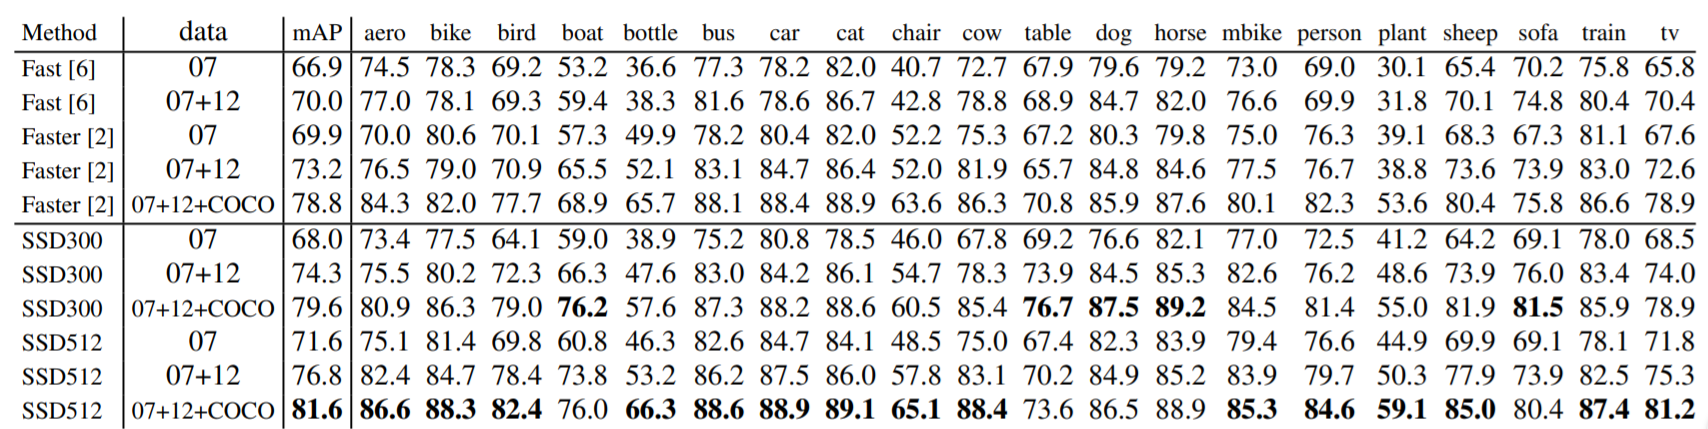
\includegraphics[width=15cm]{Bilder/ssd_results_details.png} 
		\caption[SSD Grundprinzip]{SSD Grundprinzip \cite{ssd.20161229}}
		\label{amountofdata}
	\end{center}
\end{figure}

Unter Hinzunahme des COCO \textit{trainval135k} Datensatzes erreicht der \textit{SSD} sogar das beste Ergebnis aus der ursprünglichen Veröffentlichung (siehe Abbildung \ref{amountofdata}) \cite{ssd.20161229}. 

\subsection{Techniken zur Verbesserung von Trainingsergebnissen}

Datenaugmentierung und Transfer-Learning
